% !TEX encoding = UTF-8
% !TEX TS-program = pdflatex
% !TEX root = ../tesi.tex

%**************************************************************
\chapter{Descrizione dello stage e obiettivi}
\label{cap:Descrizione dello stage e obiettivi}
%**************************************************************

\intro{In questo capitolo viene introdotto il progetto e viene descritto come è stato organizzato il lavoro in azienda con gli obiettivi iniziali e le variazioni rispetto a quanto pianificato inizialmente.}\\

%**************************************************************
\section{Introduzione al progetto e scopo}
Lo scopo del progetto di stage è lo sviluppo di una piattaforma web-mobile per la gestione di eventi sportivi. È stata effettuata una fase iniziale di analisi e progettazione, basata sull’utilizzo del framework Flutter in linguaggio Dart, seguita dalla realizzazione di alcune parti dell’interfaccia mobile.
Regolarmente, ci sono stati incontri diretti con il tutor aziendale Fabio Pallaro per verificare lo stato di avanzamento, chiarire eventualmente gli obiettivi, affinare la ricerca e aggiornare il piano di lavoro.

\section{Obiettivi dello stage}
Come obiettivi è stato richiesto di:
\begin{enumerate}
	\item Realizzare le funzionalità indicate;
	\item Produrre un documento Tecnico che descriva le funzionalità realizzate;
	\item Rilasciare il codice sul repository che verrà indicato dall’azienda.\\
	
\end{enumerate}
\subsection*{Notazione}
Per gli obiettivi delle stage si farà riferimento ai requisiti secondo le seguenti notazioni:
\begin{itemize}
	\item \textit{O} per i requisiti obbligatori, vincolanti in quanto obiettivo primario richiesto dal committente;
	\item \textit{D} per i requisiti desiderabili, non vincolanti o strettamente necessari,
	ma dal riconoscibile valore aggiunto;
	\item \textit{F} per i requisiti facoltativi, rappresentanti valore aggiunto non strettamente 
	competitivo.
\end{itemize}

Le sigle precedentemente indicate saranno seguite da una coppia sequenziale di numeri, identificativo del requisito.

\subsection*{Obiettivi fissati}
Si prevede lo svolgimento dei seguenti obiettivi:
\begin{itemize}
	\item Obbligatori
	\begin{itemize}
		\item	O01: Acquisizione delle competenze sulle tematiche sopra descritte e sulle attività svolte; \\
		\item O02: Capacità di raggiungere gli obiettivi richiesti in autonomia seguendo il cronoprogramma;\\
		\item O03: Portare a termine le implementazioni previste con una percentuale di superamento pari all’80\%.\\
	\end{itemize}
	
	\item Desiderabili 
	\begin{itemize}
		\item D01: Portare a termine le implementazioni previste con una percentuale di superamento pari al 100\%.\\
	\end{itemize}
	
	\item Facoltativi
	\begin{itemize}
		\item F01:  Realizzazione di una nuova funzionalità per l'app che prevede la gestione Signin con il protcollo Oath2.\\
	\end{itemize} 
\end{itemize}

\section{Pianificazione del lavoro svolto}
In questa sezione viene mostrato come è stato il pianificato il lavoro e le variazioni apportate in seguito agli incontri regolari con il tutor aziendale Fabio Pallaro.
\subsection{Pianificazione iniziale}
All'inizio è stata fatta una pianificazione iniziale basata su 8 settimane con una pianificazione di 40 ore per ciascuna settimana per un totale di 320 ore.
La pianificazione iniziale è la seguente:
 \begin{itemize}
	\item \textbf{Prima Settimana (40 ore)}
	\begin{itemize}
		\item Presentazione strumenti di lavoro per la condivisione del materiale di studio e per la gestione
		dell’avanzamento;
		\item Condivisione scaletta di argomenti;
		\item Ripasso del linguaggio Java SE;
		\item Ripasso concetti Web (Servlet, servizi Rest, Json ecc.).
	\end{itemize}
	\item \textbf{Seconda Settimana (40 ore)} 
	\begin{itemize}
		\item Studio principi generali di Flutter e linguaggio Dart;
		\item Studio delle best practice Flutter;
		\item Studio delle architetture per i services in Flutter.
	\end{itemize}
	\item \textbf{Terza Settimana (40 ore)} 
	\begin{itemize}
		\item Studio dei widget in Flutter;
		\item Studio del prototipo di app SportWill oggi esistente.
	\end{itemize}
	\item \textbf{Quarta Settimana (40 ore)} 
	\begin{itemize}
		\item Implementazione del login/signup con salvataggio credenziali su localStorage con aggiunta di foto ed altre info dell'utente corrente;
		\item Modifica dell'interfaccia grafica nella visualizzazione 'Elenco Uscite' con filtri di ricerca.
	\end{itemize}
	\item \textbf{Quinta Settimana (40 ore)} 
	\begin{itemize}
		\item Modifica funzionalità 'Modifica Uscita';
		\item Implementazione della funzionalità 'Inserisci mappa percorso';
		\item Implementazione della funzionalità 'Uscita in esecuzione/archiviata'.
	\end{itemize}
	\item \textbf{Sesta Settimana (40 ore)} 
	\begin{itemize}
		\item Implementazione della funzionalità 'WaitForMe' per le uscite in esecuzione.
	\end{itemize}
	\item \textbf{Settima Settimana (40 ore)} 
	\begin{itemize}
		\item Termine implementazione funzionalità 'WaitForMe'.
	\end{itemize}
	\item \textbf{Ottava Settimana (40 ore)} 
	\begin{itemize}
		\item Termine integrazioni e collaudo finale.
	\end{itemize}
\end{itemize}
\newpage
La pianificazione iniziale, in termini di quantità di ore di lavoro, è stata così distribuita:
\begin{center}
\begin{table}[h!]
	
	\label{tab:Tabella riassuntiva della pianificazione iniziale di stage}
	\begin{tabularx}{\textwidth}{|c|X|}
		
		\hline
		\textbf{Durata in ore} & \textbf{Descrizione dell'attività} \\\hline
		
		\textbf{40} & \textbf{Formazione sulle tecnologie} \\	 
		\hline
		
		\textbf{80} & \textbf{Definizione architettura di riferimento e relativa documentazione} \\  \hdashline
		\multirow{3}{0cm}\\ 
		\textit{13} & 
		\textit{Studio principi generali di Flutter e linguaggio Dart} \\
		\textit{13} & 
		\textit{Studio delle best practice Flutter} \\
		\textit{14} & 
		\textit{Studio delle architetture per i services in Flutter} \\
		\textit{20} & 
		\textit{Studio dei widget in Flutter} \\
		\textit{20} & 
		\textit{Studio del prototipo di app SportWill oggi esistente} \\
		\hline
		\textbf{160} & \textbf{Implementazioni} \\ \hdashline
		\multirow{3}{0cm}\\ 
		\textit{20} & 
		\textit{Implementazione del login/signup con salvataggio credenziali su localStorage con aggiunta di foto ed altre info dell’utente corrente} \\
		\textit{20} & 
		\textit{Modifica dell’interfaccia grafica nella visualizzazione ’Elenco Uscite’ con filtri di ricerca} \\
		\textit{10} & 
		\textit{Modifica funzionalità ’Modifica Uscita’} \\
		\textit{15} & 
		\textit{Implementazione della funzionalità ’Inserisci mappa percorso’} \\
		\textit{15} & 
		\textit{Implementazione della funzionalità ’Uscita in esecuzione/archiviata’} \\
		\textit{40} & 
		\textit{Implementazione della funzionalità ’WaitForMe’ per le uscite in esecuzione.} \\
		\textit{40} & 
		\textit{Termine implementazione funzionalità ’WaitForMe’} \\
		\hline
		
		\textbf{40} & \textbf{Termine integrazioni e collaudo finale.}  \\ 
		\hline
		
		\hline
		\textbf{Totale ore: 320} &  \\\hline	
	\end{tabularx}
	\vspace{0.3cm}
	\caption{Tabella riassuntiva della pianificazione iniziale di stage}
\end{table}
\end{center}
\subsection{Variazioni}
Rispetto all'inizio sono variate solamente le funzionalità da realizzare in quanto quelle già presenti sono state suddivise con un altro stagista.
Le variazioni in particolar modo sono dalla quarta alla settima settimana e sono le seguenti:
\begin{itemize}
\item \textbf{Quarta Settimana (40 ore)} 
\begin{itemize}
	\item Configurazione iniziale;
	\item Modifica logo;
	\item Modifica dell'interfaccia grafica nella visualizzazione 'Elenco Uscite' con filtri di ricerca.
\end{itemize}
\item \textbf{Quinta Settimana (40 ore)} 
\begin{itemize}
	\item Modifica funzionalità 'Modifica Uscita' con vari fix e cambio colori;
	\item Implementazione della funzionalità 'Visualizza mappa percorso'.
\end{itemize}
\item \textbf{Sesta Settimana (40 ore)} 
\begin{itemize}
	\item Implementazione della funzionalità che permette di vedere la mappa a schermo intero;
	\item Implementazione della funzionalità che permette l'aggiornamento automatico della mappa.
\end{itemize}
\item \textbf{Settima Settimana (40 ore)} 
\begin{itemize}
	\item Modifica dell'interfaccia grafica nella visualizzazione 'Elenco Uscite' con filtri di ricerca avanzati.
\end{itemize}
\end{itemize}
La pianificazione, in termini di quantità di ore di lavoro dopo la variazione è stata così distribuita:
\begin{center}
	\begin{table}[h!]
		
		\label{tab:Tabella riassuntiva della pianificazione di stage con variazioni}
		\begin{tabularx}{\textwidth}{|c|X|}
			
			\hline
			\textbf{Durata in ore} & \textbf{Descrizione dell'attività} \\\hline
			
			\textbf{40} & \textbf{Formazione sulle tecnologie} \\	 
			\hline
			
			\textbf{80} & \textbf{Definizione architettura di riferimento e relativa documentazione} \\  \hdashline
			\multirow{3}{0cm}\\ 
			\textit{13} & 
			\textit{Studio principi generali di Flutter e linguaggio Dart} \\
			\textit{13} & 
			\textit{Studio delle best practice Flutter} \\
			\textit{14} & 
			\textit{Studio delle architetture per i services in Flutter} \\
			\textit{20} & 
			\textit{Studio dei widget in Flutter} \\
			\textit{20} & 
			\textit{Studio del prototipo di app SportWill oggi esistente} \\
			\hline
			\textbf{160} & \textbf{Implementazioni} \\ \hdashline
			\multirow{3}{0cm}\\
			\textit{15} & 
			\textit{Configurazione iniziale} \\ 
			\textit{5} & 
			\textit{Modifica logo} \\ 
			\textit{20} & 
			\textit{Modifica dell’interfaccia grafica nella visualizzazione ’Elenco Uscite’ con filtri di ricerca} \\
			\textit{10} & 
			\textit{Modifica funzionalità 'Modifica Uscita' con vari fix e cambio colori} \\
			\textit{30} & 
			\textit{Implementazione della funzionalità 'Visualizza mappa percorso'} \\
			\textit{10} & 
			\textit{Implementazione della funzionalità che permette di vedere la mappa a schermo intero} \\
			\textit{30} & 
			\textit{Implementazione della funzionalità che permette l'aggiornamento automatico della mappa.} \\
			\textit{40} & 
			\textit{Modifica dell'interfaccia grafica nella visualizzazione 'Elenco Uscite' con filtri di ricerca avanzati.} \\
			\hline
			\textbf{40} & \textbf{Termine integrazioni e collaudo finale.}  \\ 
			\hline
			\hline
			\textbf{Totale ore: 320} &  \\\hline	
		\end{tabularx}
		\vspace{0.3cm}
		\caption{Tabella riassuntiva della pianificazione di stage con variazioni}
	\end{table}
\end{center}
\newpage
\section{Strumenti di comunicazione per lo svolgimento del lavoro}
Per ottimizzare lo svolgimento del lavoro sono stati usati i seguenti strumenti di comunicazione:
\begin{itemize}
	\item \textbf{Trello} che mi ha permesso organizzare e gestire il progetto tramite la creazione di una bacheca condivisibile;
	\begin{figure}[htbp]	
		\centering
		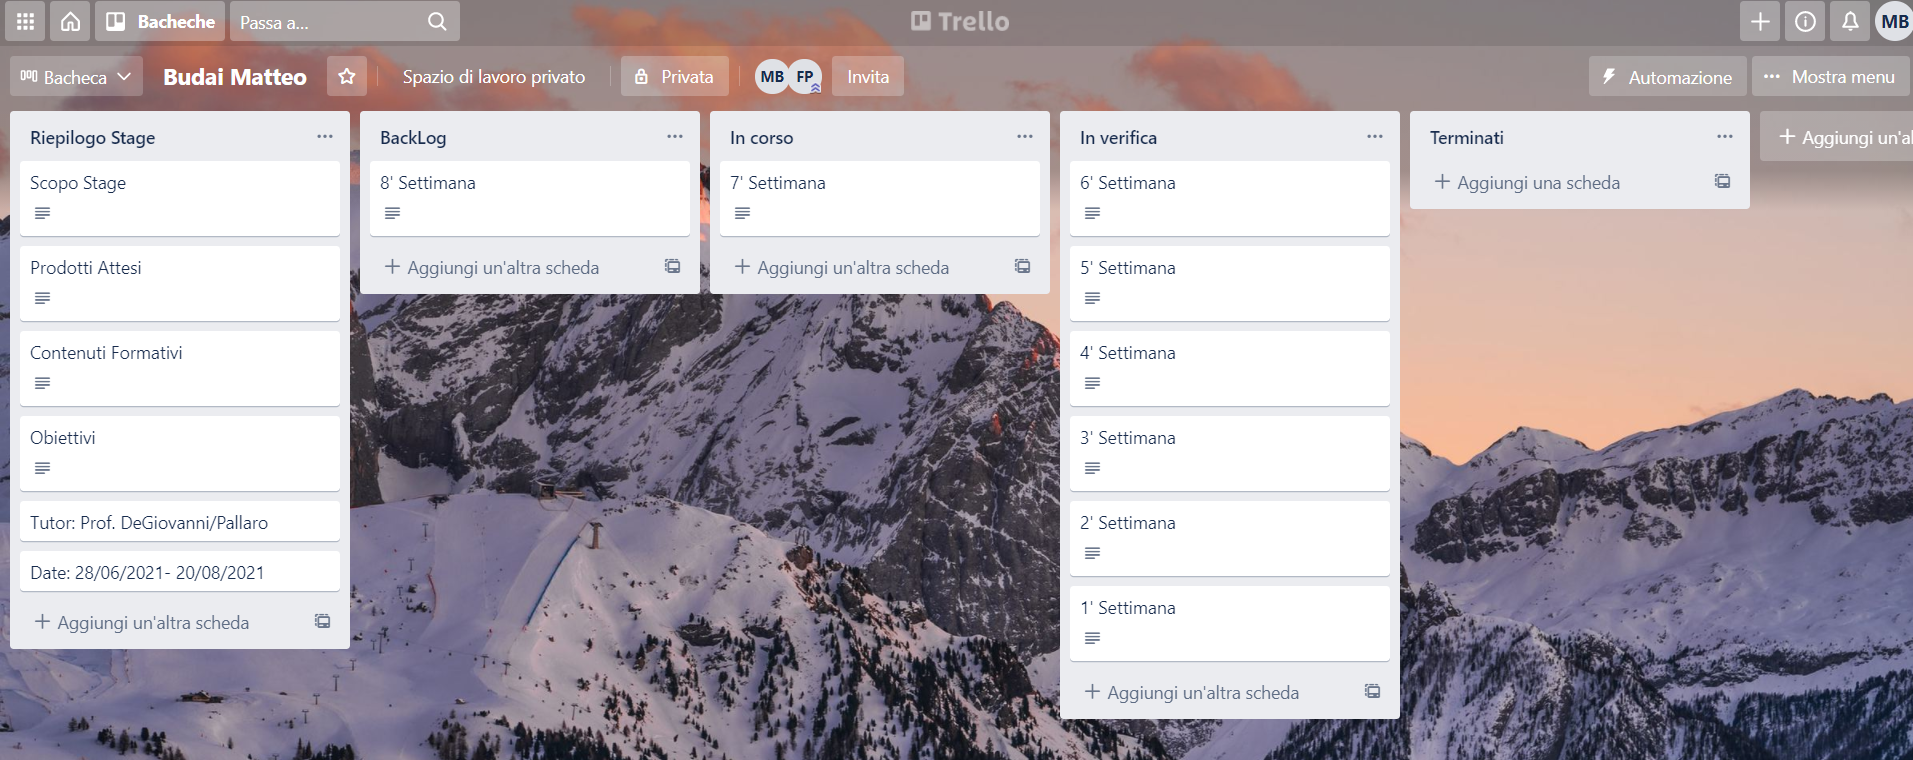
\includegraphics[width=8cm]{immagini/trello.png}
		\caption{Trello}
		\label{fig:Trello}
	\end{figure}
	\item \textbf{Google sheets} in cui venivano riportate ogni giorno le attività che si andavano a svolgere. Veniva segnalato con una spunta se l'attività era corretta oppure nella colonna aggiustamenti veniva spiegato in che modo o cosa svolgere;
	\begin{figure}[htbp]	
		\centering
		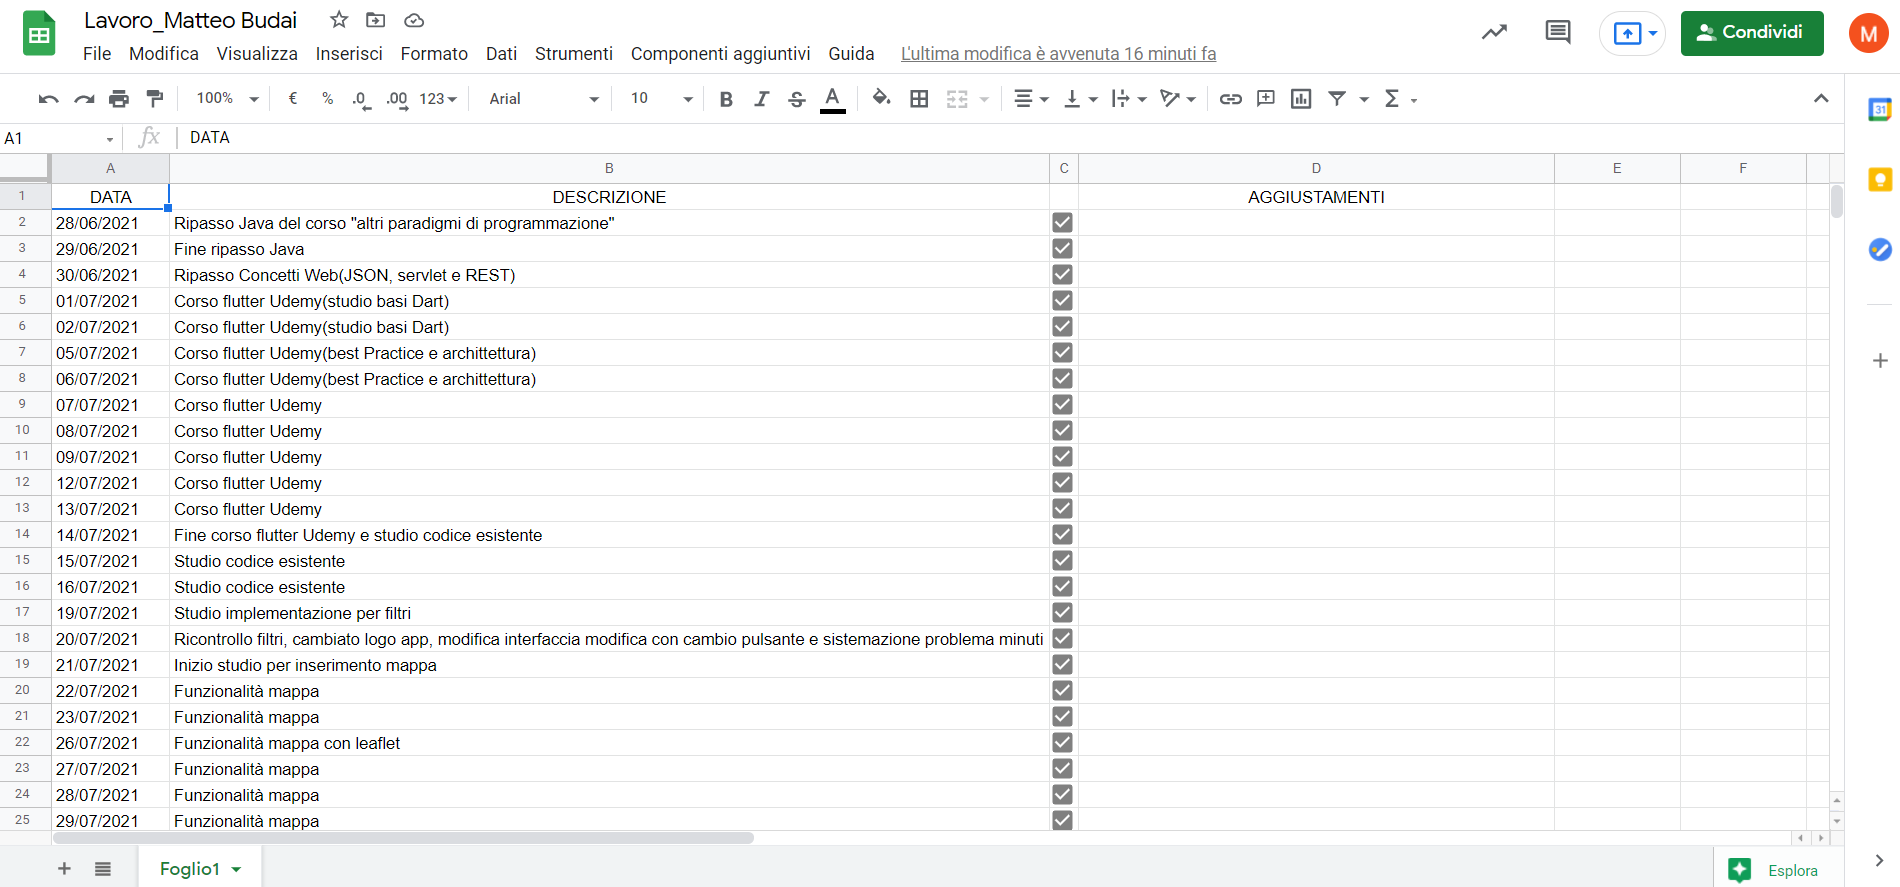
\includegraphics[width=8cm]{immagini/googlesheet.png}
		\caption{Google sheets}
		\label{fig:Google sheets}
	\end{figure}
	\item \textbf{Discord} che mi ha permesso di interfacciarmi direttamente
	con il tutor aziendale sfruttando più canali di comunicazione vocali e testuali, divisi per argomenti.
\end{itemize}
	


